\documentclass[10pt,a4paper]{article}
\usepackage[utf8]{inputenc}
\usepackage[danish]{babel}
\usepackage{amsmath}
\usepackage{hyperref}
\usepackage{amsfonts}
\usepackage{amssymb}
\usepackage{graphicx}
\author{Anders Christian Ketelsen, s133195 Gustav Valdemar Fjorder, s153651 Philip August Kisling s164421}
\title{Boblesortering}
\begin{document}
\maketitle
\begin{abstract}
Dette dokument omhandler boblesortering. Der beskrives algoritmen og præsenteres en kompleksitetsanalyse.
\end{abstract}
\section{Introduktion}

Boblesortering (\textsl{eng. bubble sort}) er en populær sorteringsalgoritme og er en af de simpleste algoritmer at forstå og implementere. Dog er den ikke en særlig effektiv sorteringsalgoritme\footnote{Mere om dette i ``Algoritmer og Dataskruturer 1''}; hverken for store eller små lister, og den anvendes sjældent i praksis. Boblesortering sorterer, som navnet antyder, elementerne i en liste ved at \textsl{boble} hvert element gennem listen til sin plads i listen.


\subsection{Pseudokode}
Wikipedia \cite{wiki} giver følgende pseudokode for boblesortering.
\begin{verbatim}
procedure bubbleSort( A : list of sortable items ) defined as:
  do
    swapped :=false
    for each i in 0 to length(A) - 2 inclusive do:
      if A[i] > A[i+1] then
        swap( A[i], A[i+1] )
        swapped := true
      end if
    end for
  while swapped
end procedure
\end{verbatim}


\section{Analyse af boblesortering}
Antallet af sammenligninger, som boblesortering udfører på en tabel af længde $n$, er i værste fald
\[\sum_{i=1}^{n-1}i=1+2+3+...+n-1=\frac{n(n-1)}{2}\]
I bedste fald er antallet $n-1$. Se tabel \ref{table:Boblesortering}.
\newpage

\begin{figure}
\centering
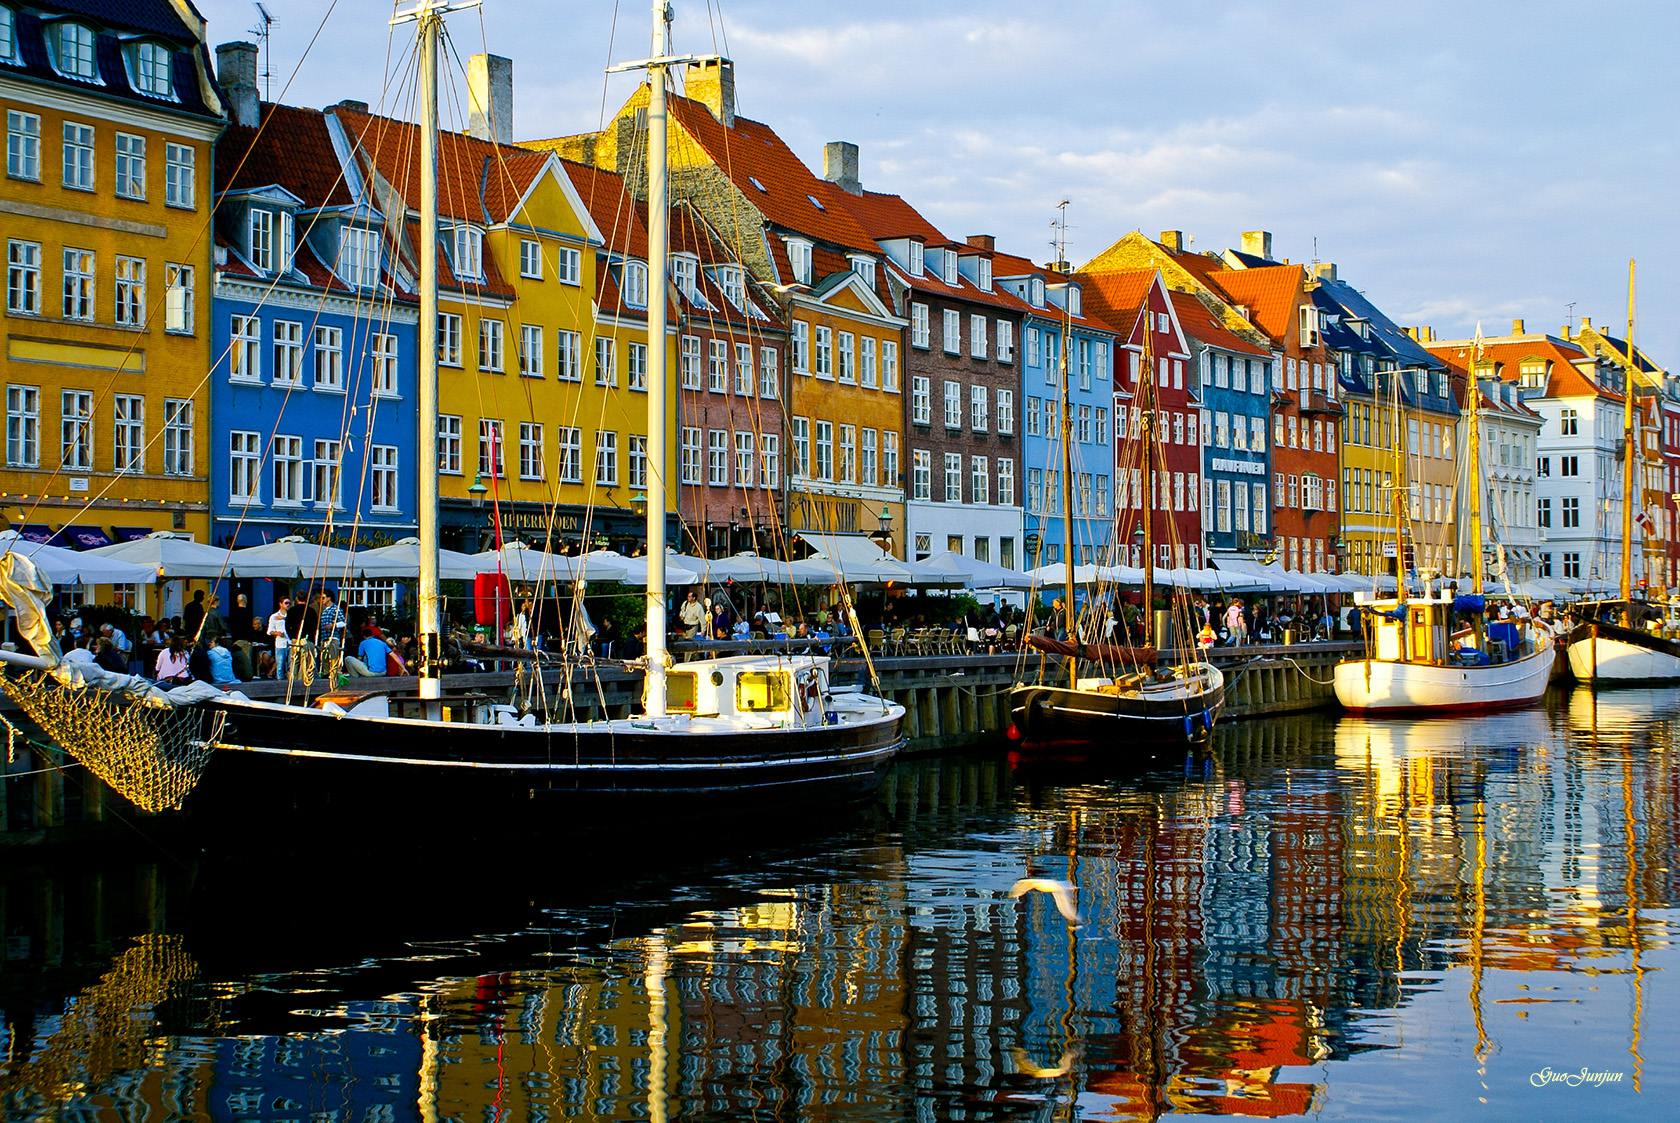
\includegraphics[scale=0.5]{Nyhavn1}\caption{Illustration af boblesortering.}\label{fig:nyhavn}
\end{figure}

\begin{table}[]
\centering
\label{table:Boblesortering}
\begin{tabular}{|l|l|}
\hline
\textbf{Værst} & $n(n-1)/2$  \\ \hline
\textbf{Bedst} & $n-1$ \\ \hline
\end{tabular}
\caption{Antal sammenligninger for boblesortering.}
\end{table}

\section{Videre læsning}
For en komplet introduktion til boblesortering og relaterede sorteringsalgoritmer se Knuth \cite{pa}.

\begin{thebibliography}{99}
\bibitem{pa} Donald Knuth. The Art og Computer Programming, Volume~3. Addison-Wesley.
\bibitem{wiki} \url{http://en.wikipedia.org/wiki/Bubble_sort}
\end{thebibliography}
\end{document}